 
% Para una visualizacion correcta, generar el PDF
% Ni el DVI ni el PS se visualizan bien

% Elegir el estilo que se desee, hay cientos en la red

\documentclass[12pt]{beamer}
%\usetheme{Warsaw}
\usetheme{JuanLesPins}
\usepackage[galician]{babel}
% \usepackage[spanish]{babel}
\usepackage[utf8]{inputenc}
%\usepackage[latin1]{inputenc}
\usepackage{makecell}

\begin{document}
\title{Deseño dunha linguaxe orientada ao xogo de rol en liña}
%\subtitle{Grao en Enxeñaría Informática}  
\author[Martín Coego Pérez]{Autor: Martín Coego Pérez \\
Director: Paulo Félix Lamas \\
Co-director: Tomás Teijeiro Campo}
\institute[USC]{Universidade de Santiago de Compostela \\[\medskipamount]

\includegraphics[height=2cm]{figuras/logo_usc-eps-converted-to.pdf}}
\date[2017]{22 de febreiro do 2017}

\AtBeginSection[]
{
  \begin{frame}[plain]
    \frametitle{Táboa de contidos}
    \tableofcontents[currentsection,hideallsubsections]
  \end{frame}
}



\begin{frame}[plain]
\titlepage
\end{frame}


%\begin{frame}[plain]
%\frametitle{Táboa de contidos}
%\tableofcontents[hideallsubsections]
%\end{frame} 

\section{Introdución}

\subsection{Obxectivos e xustificación do proxecto}
\begin{frame}
\frametitle{Motivación do proxecto}
\begin{block}{Motivación principal}
Deseñar unha linguaxe de script propia orientada á xestión de partidas de rol,
permitindo definir o sistema de xogo, crear o mundo da partida e poboalo de
obxectos.
\end{block}
\begin{block}{Obxectivos xerais}
Implementar un intérprete da linguaxe, un motor de xogo que manteña os datos da
partida, e desenvolver unha interface web accesible para os usuarios.
\end{block}
\end{frame}

\subsection{Os xogos de rol}
\begin{frame}
\frametitle{Os xogos de rol}
\begin{block}{Concepto do xogo de rol}
Xogo de interpretación entre varios xogadores que elaboran unha narrativa común,
identificándose cada xogador cun personaxe.
\end{block}
\begin{itemize}
\item Un xogador adopta o papel de \alert{Director de Xogo}
\item Os demais xogadores interpretan aos seus personaxes
\end{itemize}


\includegraphics[height=1cm]{figuras/presentacion/dungeonsanddragons_logo.jpg}

\includegraphics[height=1cm]{figuras/presentacion/call-of-cthulhu-logo.png}

\includegraphics[height=1cm]{figuras/presentacion/Vampirethemasquerade-logo.png}
\end{frame}

\subsection{Ferramentas informáticas existentes}
\begin{frame}
\frametitle{Ferramentas informáticas existentes}
\begin{columns}[T]
\begin{column}[T]{5cm}
\begin{figure}
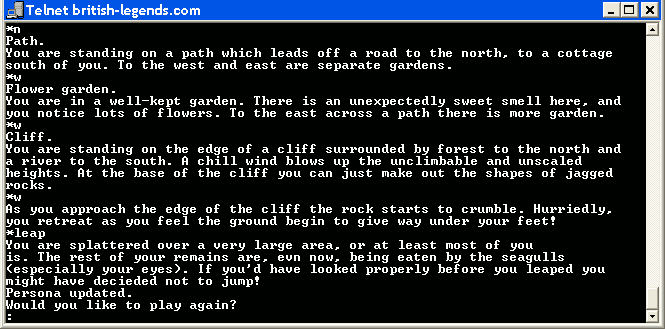
\includegraphics[height=2.5cm]{figuras/presentacion/MUD1_screenshot.png} \\
\end{figure}
\begin{figure}
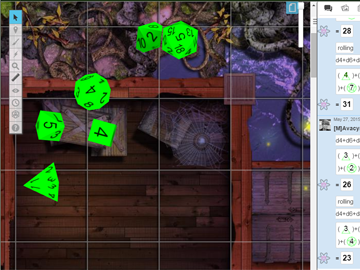
\includegraphics[height=2.5cm]{figuras/presentacion/roll20.png}
\end{figure}
\end{column}
\begin{column}[T]{5cm}
\begin{figure}
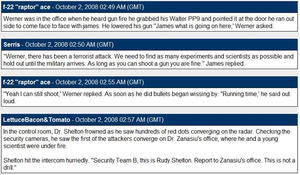
\includegraphics[height=2.5cm]{figuras/presentacion/300px-Darwin's_Soldiers_image.png} \\
\end{figure}
\begin{figure}
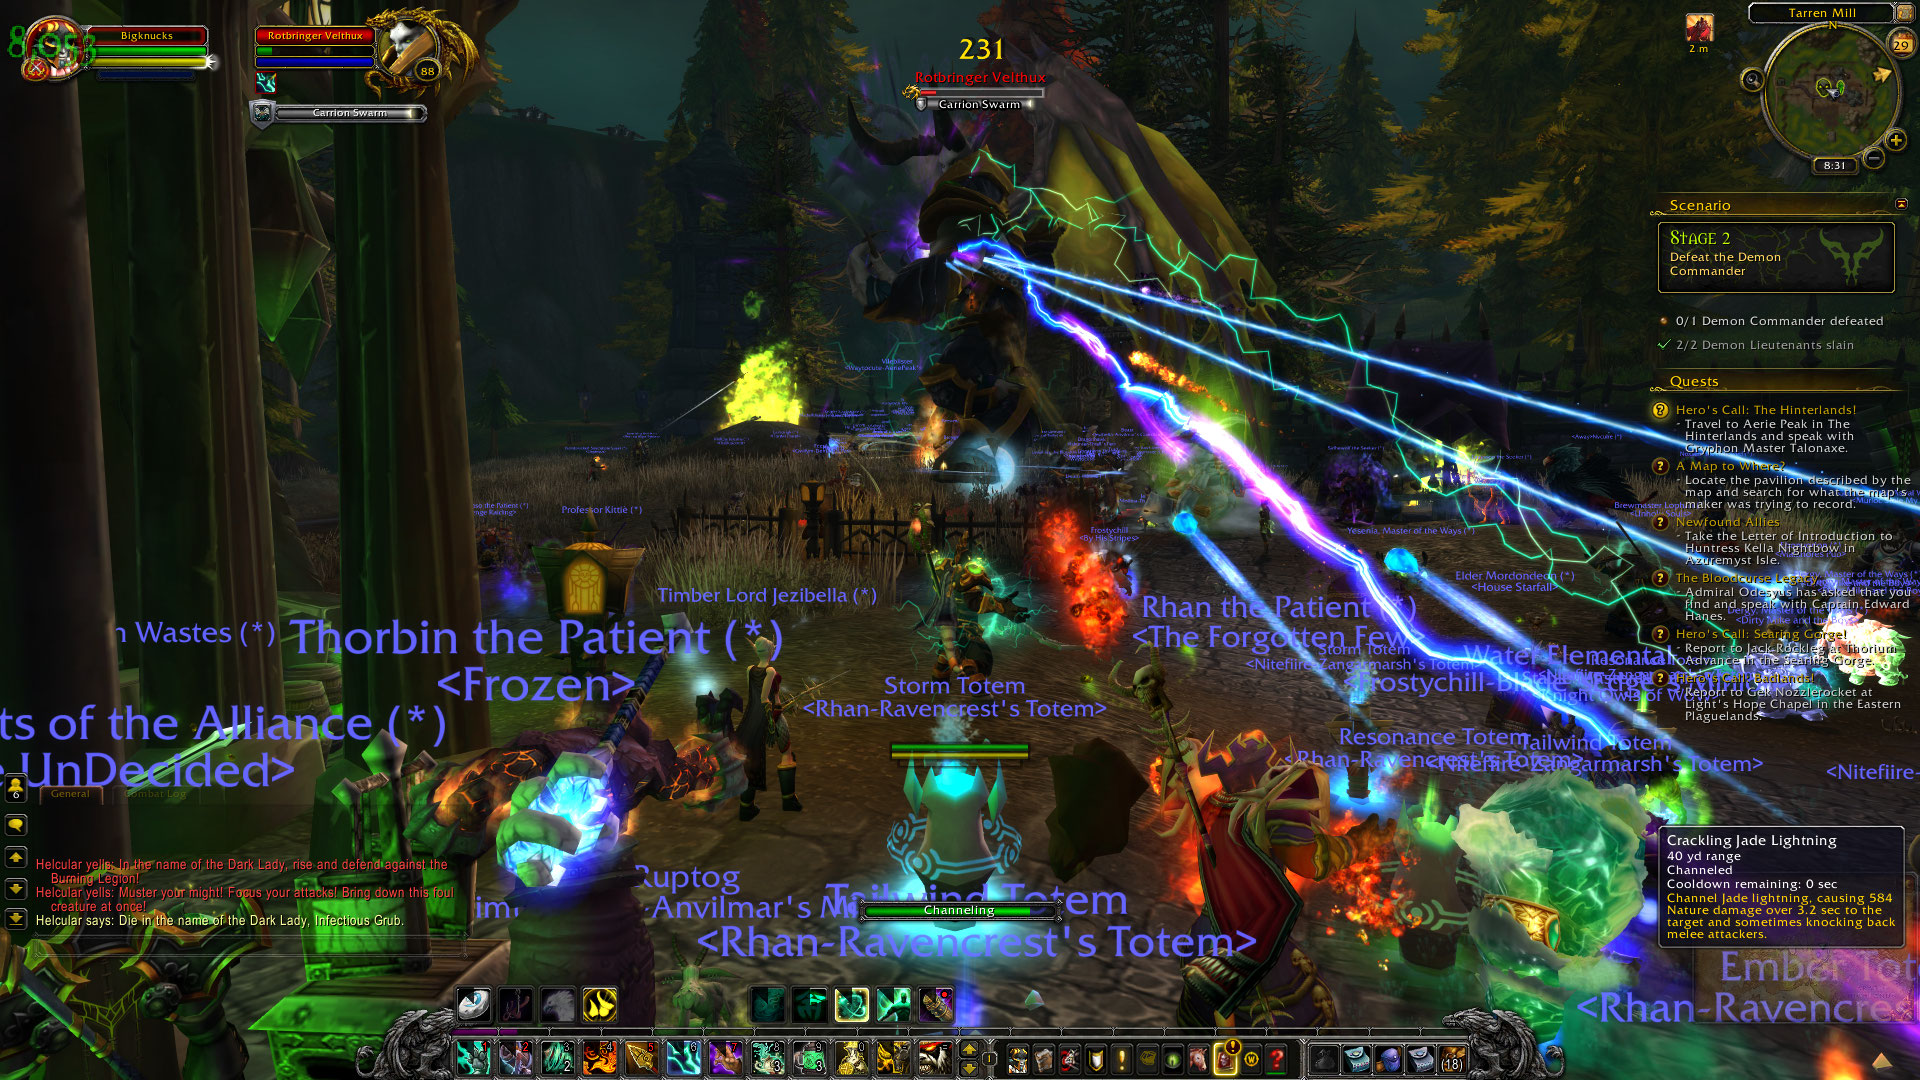
\includegraphics[height=2.5cm]{figuras/presentacion/WoW-4.jpg}
\end{figure}
\end{column}
\end{columns}
\end{frame}

\subsection{Metodoloxía de desenvolvemento}
\begin{frame}
\frametitle{Metodoloxía SCRUM}
\begin{block}{Características do proxecto}
Aborda un dominio con escasas aportacións tecnolóxicas, polo que se intúen
numerosos cambios nos requisitos do proxecto. Experiencia escasa do autor en
proxectos grandes.
\end{block}
\begin{block}{Por que SCRUM}
Metodoloxía áxil mediante iteracións, permite facer cambios en calquera etapa do
proxecto.
\end{block}
\end{frame}

\section{Análise}

\subsection{Definicións}
\begin{frame}
\frametitle{Principais definicións do sistema}
\begin{block}{Decisión}
Descrición verbal dun xogador explicando a acción que pretende que realice
o seu personaxe.
\end{block}

\begin{block}{Acción}
Conxunto de liñas de código que alterarán o mundo de xogo nun determinado
escenario.
\end{block}

\begin{block}{Narración}
Texto redactado polo DX asociado a unha determinada acción.
\end{block}
\end{frame}

\subsection{Obtención de requisitos}

\begin{frame}
\frametitle{Requisitos}
\begin{block}{Requisitos funcionais}
Unha parte importante dos requisitos funcionais fan referencia a funcionalidades
propias da linguaxe de script a deseñar.
\end{block}
\begin{tabular}{| l | l | }
\hline
Alta de usuarios & \alert{Eliminación de obxectos} \\
Modificación de usuarios & \alert{Ligazón personaxe-xogador} \\
Identificación de usuarios & Creación dun escenario \\
\alert{Creación de clases} & Eliminación dun escenario \\
\alert{Modificación de clases} & \alert{Cambio de escenario de obx.} \\
Eliminación de clases & Envío de decisións \\
\alert{Creación de obxectos} & Visualización de narracións \\
\alert{Modificación de obxectos} & \\
\hline
\end{tabular}
\end{frame}

\section{Arquitectura e ferramentas}
\subsection{Bloques da arquitectura}

\begin{frame}[plain]
\frametitle{Arquitectura do sistema}
\begin{figure}
\includegraphics[scale=0.3]{figuras/diagramas/arquitectura.pdf} 
\end{figure}
\end{frame}

\begin{frame}
\frametitle{Diagrama de secuencia}
\begin{figure}
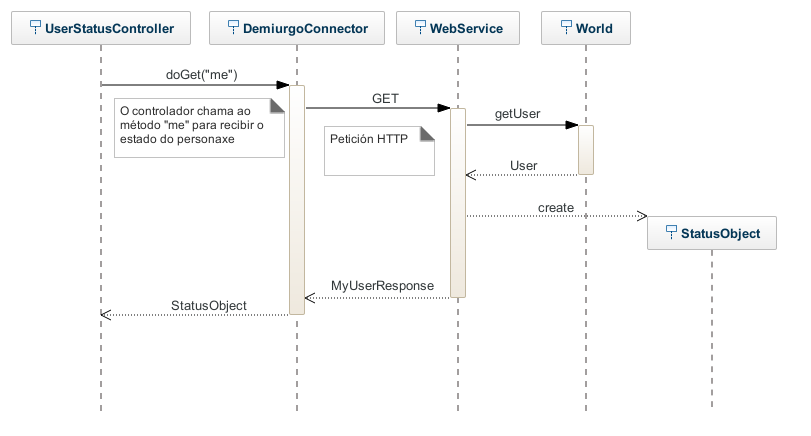
\includegraphics[scale=0.5]{figuras/diagramas/secuencia.png} 
\end{figure}
\end{frame}

\subsection{Linguaxe de script} 

\begin{frame}
\frametitle{Linguaxe COE}
\begin{block}{COE}
COE, Acrónimo de \textit{Código de Obxectos e Escenarios}, é a linguaxe de
script empregada polo DX para \alert{interactuar co mundo de xogo}. 
\end{block}
\begin{block}{Características}
É unha linguaxe \alert{orientada a obxectos} cun deseño centrado na xestión
dunha partida de rol, tanto na definición do mundo como no transcurso da
partida.
\end{block}
\begin{block}{Implementación}
Elaborouse unha \alert{gramática} que contén a definición formal da linguaxe, da
que se partiu para facer un intérprete de código.
\end{block}
\end{frame}

\subsection{Análise tecnolóxica} 
\begin{frame}
\frametitle{Tecnoloxías empregadas máis relevantes}
\begin{block}{ANTLR}
Xera un analizador sintáctico a partir dunha gramática dada.
\end{block}

\begin{block}{Servizos REST}
Interface de comunicación entre aplicacións a través de peticións HTTP.
\end{block}

\begin{block}{Spring Framework}
Framework de desenvolvemento de aplicacións Java.
\end{block}
\end{frame}

\section{Deseño}

\subsection{Deseño da linguaxe COE}
\begin{frame}
\frametitle{Principais consideracións}
\begin{block}{Tipos de entrada}
A linguaxe acepta dous tipos de entrada diferenciados:
\begin{itemize}
  \item Código de definición de clase
  \item Código regular de acción
\end{itemize}
\end{block}
\begin{columns}[T]
\begin{column}[T]{5cm}
\begin{exampleblock}{Ex. definición de clase}
\begin{figure}
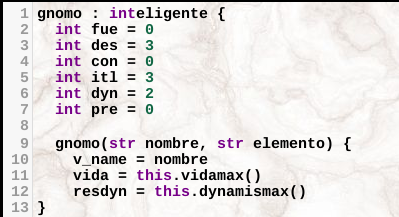
\includegraphics[scale=0.4]{figuras/presentacion/demiugo_gnomo.png} 
\end{figure}
\end{exampleblock}
\end{column}
\begin{column}[T]{5cm}
\begin{exampleblock}{Ex. código de acción}
\begin{figure}
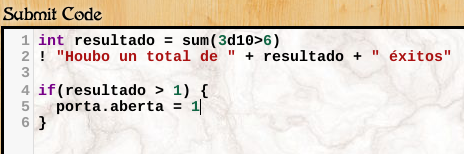
\includegraphics[scale=0.4]{figuras/presentacion/demiurgo_accion.png} 
\end{figure}
\end{exampleblock}
\end{column}
\end{columns}
\end{frame}

\begin{frame}
\frametitle{Características da linguaxe}
\begin{block}{Herdanza de clases}
As clases poden ser fillas doutras clases, herdando campos e métodos. Existe o
polimorfismo de campos e métodos.
\end{block}

\begin{block}{Sistema de tipos}
COE é unha linguaxe fortemente tipada: as variables deben declararse
especificando o seu tipo de dato. Isto reduce o impacto dos erros na
codificación.
\end{block}
\end{frame}

\begin{frame}
\frametitle{Scope}
\begin{block}{Scopes}
Cada scope correspóndese cun contexto dentro do código, e xestiona as
declaracións e invocacións de variables no código relacionándoas co elemento
correspondente do modelo de datos.
\end{block}
\begin{exampleblock}{Exemplo}
FunctionScope créase ao executar unha función. Ao declarar novas variables,
estas serán locais dentro na función, e se eliminarán unha vez esta remate.
\end{exampleblock}
\end{frame}

\begin{frame}
\frametitle{Implementación: Patrón Visitor}
\begin{block}{Patrón Visitor}
A implementación da lóxica da linguaxe COE realizouse empregando o patrón
Visitor, que permite percorrer unha árbore sintáctica e definir a semántica
de cada nodo da mesma.
\end{block}

\begin{block}{Clases Visitor}
No software hai dúas clases Visitor definidas: unha para definicións de clases e
outra para código de accións, xa que os dous modos teñen diferencias á hora de
interpretar o código.
\end{block}
\end{frame}

%%%%%%%%%%%%%%%%%%%%%%%%%%%%%%%%%%%%%%%%%%%%%%%%%%%%%%%%%%%
\section{Demostración}
\begin{frame}
\frametitle{Demostración}
\begin{block}{Servidor}
É posible atopar un servidor coa plataforma en funcionamento no enderezo
\url{http://www.demiurgo.pro}, no que se realizaron as probas de usabilidade con
usuarios reais.
\end{block}
\begin{figure}
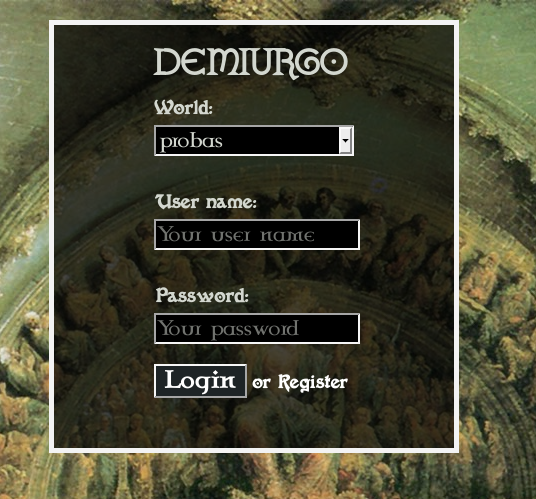
\includegraphics[scale=0.3]{figuras/presentacion/demiurgo_login.png} 
\end{figure}
\end{frame}

%%%%%%%%%%%%%%%%%%%%%%%%%%%%%%%%%%%%%%%%%%%%%%%%%%%%%%%%%%%


\section{Validación e probas}
\subsection{Implementación}
\begin{frame}
\frametitle{Principais problemas atopados}
\begin{block}{Estimación da complexidade do proxecto}
A complexidade do proxecto foi incorrectamente estimada no inicio do mesmo, o
que conlevou a imposibilidade de cumprir co prazo inicial.
\end{block}

\begin{block}{Uso de tecnoloxías novas}
A reducida experiencia do desenvolvedor nas tecnoloxías empregadas esixiu asumir
o aprendizaxe das mesmas, o que ralentizou o desenvolvemento.
\end{block}

\begin{block}{VPS}
Foi necesario buscar e configurar un servidor VPS ao final do proxecto, e isto
implicou custos económicos e de tempo.
\end{block}
\end{frame}

\renewcommand\theadfont{\bfseries}

\begin{frame}
\frametitle{Sprints}
\begin{table}
\footnotesize
\begin{tabular}{|l|r|r|}
\hline
\thead{Nome do Sprint} & \thead{Data inicio} & \thead{Data fin} \\
\hline
Análise de requisitos & 13/03/2016 & 25/04/2016 \\
\hline
Bosquexos da linguaxe & 25/04/2016 & 23/05/2016 \\
\hline
Definición formal da linguaxe & 23/05/2016 & 01/06/2016 \\
\hline
Analizador sintáctico & 01/06/2016 & 09/06/2016 \\
\hline
Implementación da linguaxe en Java & 09/06/2016 & 21/06/2016 \\
\hline
Clases e escenarios & 21/06/2016 & 19/07/2016 \\
\hline
Comprobación do input & 19/07/2016 & 08/08/2016 \\
\hline
Interacción co usuario & 08/08/2016 & 29/08/2016 \\
\hline
Servizos REST & 29/08/2016 & 19/09/2016 \\
\hline
Base da memoria & 19/09/2016 & 09/11/2016 \\
\hline
Deseño inicial da web & 09/11/2016 & 15/12/2016 \\
\hline
Apartado gráfico da interface & 15/12/2016 & 28/12/2016 \\
\hline
Inventarios e configuración & 28/12/2016 & 08/02/2017 \\
\hline
\end{tabular}
\end{table}
\end{frame}

\subsection{Probas}
\begin{frame}
\frametitle{Probas unitarias}
\begin{block}{Motor de xogo}
As probas unitarias realizáronse \alert{sobre o intérprete da linguaxe COE}.
Comproban que se executan as instrucións precisas.
\end{block}
\begin{exampleblock}{Exemplo}
Executar o código \textit{``new object()''} e comprobar se se engadiu un novo
obxecto da clase correspondente.
\end{exampleblock}
\begin{alertblock}{Execución das probas}
As probas unitarias están definidas no proceso de compilación do motor de xogo,
polo que se executan en cada nova compilación.
\end{alertblock}
\end{frame}

\begin{frame}
\frametitle{Probas de usabilidade}
\begin{block}{Cuestionarios}
As probas de usabilidade fixéronse probando a interface web con usuarios reais e
enviándolles cuestionarios para cubrir.
\end{block}
\begin{columns}[T]
\begin{column}[T]{5cm}
\begin{figure}
\includegraphics[scale=0.3]{figuras/cuestionario_dx.pdf} 
\end{figure}
\end{column}
\begin{column}[T]{5cm}
\begin{figure}
\includegraphics[scale=0.3]{figuras/cuestionario_xogador.pdf} 
\end{figure}
\end{column}
\end{columns}
\end{frame}

\section{Conclusións}
\subsection{Conclusións e ampliacións}

\begin{frame}
\frametitle{Conclusións}
\begin{block}{Ámbito do proxecto}
A plataforma desenvolvida neste proxecto cubre un espazo sen explorar dentro do
mundo dos xogos de rol. Non existen antecedentes de sistemas semellantes a este.
\end{block}

\begin{block}{Linguaxe COE}
O deseño e implementación dunha linguaxe propia para comunicarse co sistema
achega a programación informática aos xogos de rol, fomentando a adquisición de
competencias neste campo por parte dos usuarios.
\end{block}
\end{frame}

\begin{frame}
\frametitle{Posibles ampliacións}
\begin{block}{Novas formas de acceso ao sistema}
O sistema permite o desenvolvemento de terceiras aplicacións tales como
\alert{bots de Telegram} ou \textit{apps} para tableta ou móbil.
\end{block}
\begin{block}{Ampliacións da linguaxe}
Hai ampliacións da linguaxe planificadas como o engadido etiquetas de
visibilidade para os campos dos obxectos.
\end{block}
\begin{block}{Ampliacións da web}
A web pode ser mellorada con ferramentas como un \alert{chat XMPP} para
comunicarse co DX ou un xestor de temas personalizados.
\end{block}
\end{frame}

\begin{frame}
\frametitle{Formación de comunidade}
\begin{block}{Comunidade de xogadores}
\begin{itemize}
  \item Aproveitar a comunidade de rol xa existente
  \item Promoción por redes sociais
  \item Internacionalización do sistema
\end{itemize}
\end{block}
\begin{block}{Comunidade de desenvolvedores}
\begin{itemize}
  \item Licencia libre do código
  \item Repositorio Git aberto
\end{itemize}
\end{block}
\end{frame}

\end{document}